\chapter{Discovery Potential \Contact{Francis-Yan}}
\Contributors{Tony, Vera, Cora, Francis-Yan, Alex, Keith ...}
\label{sec:discovery}
\bigskip

Cosmology has a long history of testing particle models of dark matter.
%probing the fundamental properties of dark matter.
For instance, neutrinos were long considered a viable dark matter candidate \citep[\eg,][]{Kolb:1988}, and eventually, precise cosmological measurements made clear that the Universe contains multiple invisible components.
%\KB{Alternatively, the rest of this paragraph could go into a footnote.}
%For a case study of the interplay between particle physics experiments and astrophysics observations, consider the 30~eV neutrino dark matter candidate.
The 30~eV neutrino dark matter candidate is an especially interesting case study of the interplay between particle physics experiments and astrophysical observations.
\citet{Lyubimov:1980un} reported the discovery of a non-zero neutrino rest mass in the range $14 \unit{eV} < m_{\nu} < 46 \unit{eV}$ which was subsequently tested by several other tritium $\beta$-decay experiments over the next decade.
% See equation 19 of  https://arxiv.org/pdf/1212.6154.pdf
Neutrinos with this mass would provide a significant fraction of the critical energy density needed to close the universe, but would be relativistic at the time of decoupling (i.e., hot dark matter).
During the same period, the first stellar velocity dispersion results for dwarf spheroidal galaxies showed that these galaxies are highly dark matter dominated.
The inferred dark matter density within the central regions of the dwarfs
%compact region of stellar population of the dwarfs
was used to place lower limits on the neutrino rest mass that were incompatible with the 30~eV neutrino dark matter candidate \citep{Aaronson:1983,Gerhard:1992}.
%In 1980, a $\beta$-decay experiment at ITEP reported the discovery of non-zero neutrino mass in the range  \citep{Lyubimov:1980un}.
%As a specific case study, the tritium $\beta$-decay experiment at ITEP reported a neutrino mass of $\approx30$~eV for much of the 1980s \citep{Lyubimov:1980un}. Neutrinos at this mass would provide a significant fraction of the critical energy density. However, the stellar velocity dispersion of dwarf spheroidal galaxies orbiting the Milky Way, e.g., Draco \citep{Aaronson:1983}, already  }
Similar stories can be told of heavy leptons \citep{Gunn:1978}, \CHECK{and other dark matter candidates}, which have been excluded by cosmological and astrophysical measurements.
Cosmology has continually proven that it is impossible to separate the \emph{macroscopic distribution} of dark matter from the \emph{microscopic physics} governing dark matter.

% See discussion on "Outline for discovery section" 19 December 2018
% https://docs.google.com/document/d/1RaxmjYjRYaAAY-4zqg-v4bEtUa8rcgiVgnJlFJQZifc/edit#

Through much of this work, we have expressed sensitivity to dark matter microphysics in terms of upper limits in the case of non-detection of deviations from the baseline CDM paradigm.
In this Section, we consider two potential astrophysical discovery scenarios for non-minimal dark matter properties that could be realized in the LSST era.
In each scenario, a critical question is whether the systematic uncertainties associated with conventional astrophysical processes can be controlled at a level that would sufficiently compelling to guide non-gravitational dark matter searches with collider, direct, and indirect detection experiments.

%{\bf Compact Object Discovery}
\section{Compact Object Discovery}
% ADW: Need some help from Will et al.

While current constraints make it unlikely that all of dark matter is composed of compact objects, it is nearly certain that LSST will measure the mass spectrum of Galactic black holes (\figref{macho_discovery}).
In this regime, it will be necessary to test whether the observed black hole population statistics can be explained through stellar evolution, or if a novel black hole production mechanism is required (\ie, PBHs).
The discovery of an excess component to the black hole population will necessarily require a fit of the underlying population of stellar remnants and the associated astrophysical systematics. 
However, an excess of high-mass black holes ($M \gtrsim 30\Msun$) or the discover of black hole clusters \citep[\eg][]{1603.05234} could provide a smoking gun for PBH detection.
If such a PBH population is discovered, it will be possible to measure not only the fraction of dark matter in compact objects, but the compact object mass spectrum, which will in turn set constraints on the spectrum of perturbations during and after inflation \citep[\eg][]{:1702.03901}.
Knowing that some fraction of the dark matter exists as PBHs will necessitate re-interpretation of particle physics limits from direct and indirect searches.
Preferred regions of WIMP parameter space that are excluded under the assumption that all the dark matter is particles will be reopened.
Somewhat counter-intuitively, the outlook for the WIMP may be stronger in a universe where PBHs make up some fraction of the dark matter density.

\begin{figure}[t]
\centering
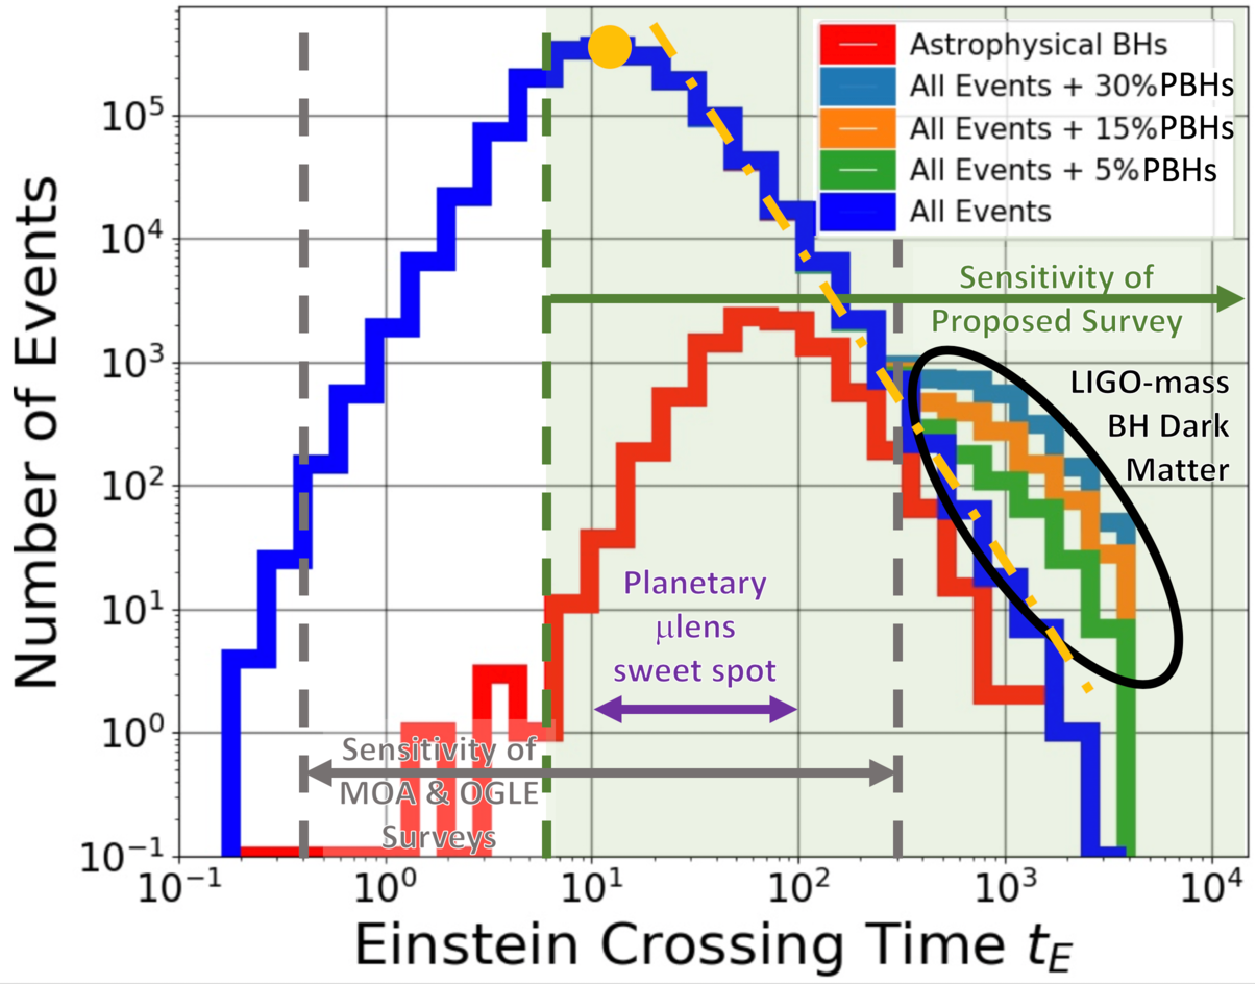
\includegraphics[width=0.6\columnwidth]{nevents_vs_t.pdf}
\caption{
    \label{fig:macho_discovery}
    The expected number of $2\theta_\mathrm{E}$ microlensing events in a $10\times10\,\mathrm{deg}^2$ bulge field (blue histogram), with the fraction due to black holes resulting from stellar evolution shown by the red histogram (for these events our detection efficiency is $\sim0.1\%$ at low-$t_\mathrm{E}$ and $\sim1\%$ at high-$t_\mathrm{E}$).
    \WAD{Need to come up with better estimates for the number of expected event, i.e., how to scale the y-axis for LSST, especially considering different regions of the sky and potentially different cadences in each of these regions. Could just present a conservative estimate for $10\times10\,\mathrm{deg}^2$ bulge field.}
    Other colored histograms show the event rate assuming different fractions of dark matter composed of LIGO-mass black holes (an order of magnitude more massive than the stellar remnant population).
    The gray vertical dashed lines show the published sensitivity ranges of the MOA and OGLE microlensing surveys (insensitive to the high-mass/long-$t_\mathrm{E}$ tail).
    The shaded green regions shows the sensitivity range for LSST.
    %This includes the planetary microlensing sweet spot (purple), which will be probed via alerted follow up.
    It also importantly includes the peak of the distribution (yellow dot), and enables us to accurately calibrate the slope (yellow dot-dashed line), which is necessary to provide accurate IMBH constraints.
    \Contributors{Jessica Lu, Casey Lam, Michael M., Will D.}
    }
\end{figure}

%{\bf SIDM-WDM Discovery}
\section{WDM/SIDM Discovery}


We now turn to the scenario in which dark matter possesses a particle mass or self-interaction cross section that would partially account for observed small-scale structure anomalies.
There are currently several hints of non-minimal dark matter particle properties arising from comparisons between theoretical predictions and observed galaxy populations at the dwarf galaxy scale, \ie, distances below $1 \Mpc$ and mass scales below $10^{11} \Msun$ \citep[reviewed by][]{BuckleyPeter:2017,Bullock:2017xww}.
However, the interpretation of these discrepancies in terms of dark matter microphysics has been hindered by present uncertainty in the mapping between visible stellar populations and dark matter halos, which involves both the physics of galaxy formation as well as the connection between observable and intrinsic galaxy properties (see \secref{smallest_galaxies} and \secref{halo_profile_group}).
In a regime where we are already limited by systematic uncertainties, it is therefore quite reasonable to ask how the increased statistical power of LSST will help to resolve our current small-scale structure quandary.

We argue here that the decisive advantage of LSST is the opportunity to combine an ensemble of astrophysical dark matter probes that offer complementary perspectives on dark matter halo abundances and profile shapes, and which are affected by different sources of systematic uncertainty.
For the purpose of illustration, we outline a possible ``roadmap to discovery'' for a dark matter model that produces as a cutoff in the matter power spectrum and a suppression of the central dark matter profile just below the current sensitivity limit---\ie, $M_{hm} = 10^{8.5}$.
As a concrete example, we assume that these astrophysical features result from a dark matter particle model with a self-interaction cross section of $\sigma/m = 0.1 \cmg$ and a thermal particle mass of $\mWDM = 6 \keV$.

The first indication of a discrepancy with CDM might come shortly after the first public data release of LSST survey data when automated searches for Milky Way satellites reveal only a handful of new candidate ultra-faint galaxies. 
Using the framework described in \secref{smallest_galaxies}, these observations could be combined to derive contours on the parameter space of WDM mass vs SIDM cross-section.
The constraints would deviate significantly from expectations derived from CDM and the observational sensitivity of LSST, thereby hinting at a preference for new physics.

The combined depth and sky coverage of LSST will also enable the study of dwarf galaxy satellite populations around other hosts out to several Mpc, as well as the ``field'' population of isolated dwarf galaxies.
By generating a statistical sample of low-luminosity galaxies in a wide variety of environments, LSST will provide a wealth of input data to theoreticians developing galaxy formation simulations.
In our hypothetical scenario, these simulations will show that it is challenging to solve the dirth of observed satellite galaxies by tuning baryonic physics models (\eg, reionization physics, supernova feedback, etc.).

The same LSST data set is expected to reveal many new stellar streams and gravitational lens systems, which would provide access to dark matter halos below the mass threshold of galaxy formation (\secref{stream_gaps} and \secref{stronglens}).
The search for stream gaps and lensing anomalies would be particularly well motivated since these systems would probe a halo mass regime where the discrepancy with CDM would be even more severe.
In addition, these halos are largely devoid of baryons and would be subject to different astrophysical and observational systematics.
We could expect a period of several years to collect and analyze follow-up observations (both spectroscopy and high-resolution imaging) of the most favorable stream and lens systems.
The absence of lower mass dark matter halos would greatly increase the tension between observations and the predictions of CDM.
In addition, it will be difficult to explain a dirth of dwarf galaxies and lower mass halos with the same astrophysical systematics, strengthening the case for a fundamental physics explanation.

In parallel, measurements of the inner density profiles of dwarf galaxies will be made using weak lensing data from LSST and with dynamical measurements from other surveys.
These measurements will start to break the model degeneracy between a minimum halo mass cutoff (\eg WDM) and an alteration to the profiles of dark matter halos (\eg SIDM).
Similarly, the (non-)observation of deviations in halo profiles of galaxy clusters will be able to inform the velocity dependence of the SIDM cross section.
Combining the LSST-discovered systems with spectroscopic follow-up and observations of the Lyman-$\alpha$ forest would result in a simultaneous measurement of a non-zero SIDM cross section and an upper limit on the WDM particle mass (\citep{sidm_wdm_disc}).
Such closed contours would signify the start of an era of precision measurement of dark matter particle properties using astrophysical observations.

\begin{figure}
\centering
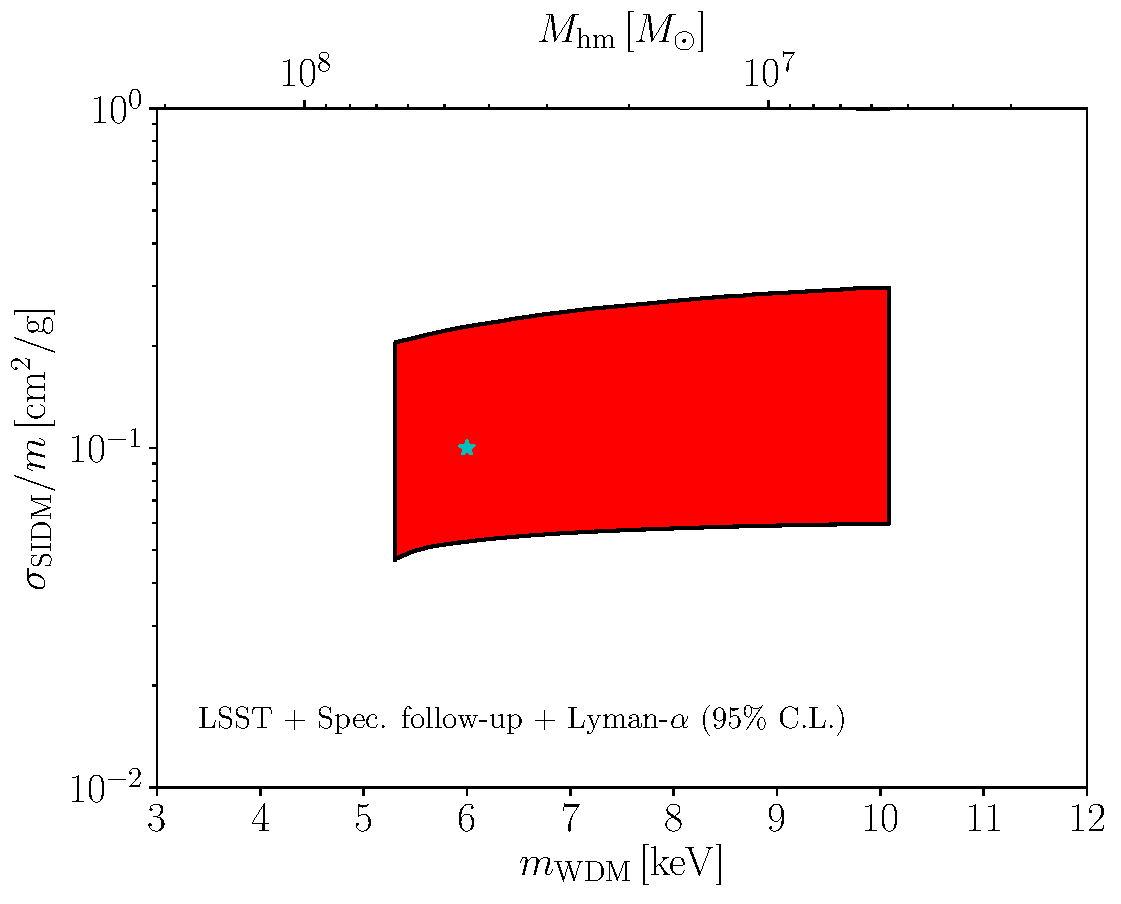
\includegraphics[width=0.6\columnwidth]{figures/SIDM_WDM_fig_disc.pdf}
\caption{\label{fig:sidm_wdm_disc} Measurement of particle properties for a dark matter model with a self-interaction cross section and thermal temperature just below current constraints ($\sigma/m = 0.1 \cmg$ and $\mWDM = 6\keV$). Contours are created by combining LSST-discovered systems with spectroscopic follow-up and measurements of the Lyman-$\alpha$ forest.
\ADW{We should make the axis range the same on this figure as the constraint figure.} \ADW{We need to add the streams...}
}
\end{figure}

%{\bf Semi-quantitative extraction of particle properties}
%As a quantitative aspect, we specifically constrain ourselves to the scenario of a dark matter model that manifests itself as a cutoff in the matter power spectrum and a suppression of the central dark matter profile. 

%We assume a maximal model where that cutoff occurs just below the current sensitivity limit---i.e., $M_{hm} = 10^{8.5}$.
%This model would manifest itself as an absence of low-mass dark matter halos detectable through measurements of Milky Way satellites, the lack of gaps in stellar streams, and an underabundance of perturbations in strongly lensed systems.

%This is the contour figure from Francis-Yan.

{\bf Roadmap to measurement}

\begin{comment}
The large advances in sensitivity enabled by LSST will open a wide range of new parameter space implying the possibility of discovery. 
We now discuss a road map from detecting anomalous signals, that misalign with the minimal CDM model, to establishing a discovery and measuring particle properties of dark matter.

There is a long history of tentatively attributing astrophysical anomalies to new dark matter physics; however, none of these have risen to a status of a confirmed discovery. 
The main reason is presence of large systematic effects that may be confused with dark matter signals, stemming from a limited understanding of processes characterizing astrophysical systems and observational biases and systematic errors. 
However, the advent of LSST (and similar surveys) offers means to largely circumvent such issues---access to a wide range of observables that may harbor signals of the same dark matter microphysics, but suffer from different systematic effects. 
Combination of orthogonal information from various probes---and measurement of a consistent signal in several of them---will be essential for establishing a discovery. 

\FIXME{This paragraph is work in progress}: As an illustration, imagine a scenario where future satellite number counts from LSST return evidence for a missing population of low-luminosity objects. 
Such measurement could imply presence of a cutoff in the matter power spectrum (as would be produced, for example, by dark matter self-interactions), but it could, alternatively, be a consequence of a lower limit on the dark matter halo mass that can host a galaxy. 
Another observable: spectroscopic follow-up measurements of the radial density profiles… [\FIXME{VG: someone else should finish this} by telling a story of how the latter measures dark matter only, so it is a direct probe of DM, but may be a lower signal-to-noise measurement; in this case, joint analysis of both observables under the SIDM hypothesis may return conclusive evidence in favor of SIDM vs CDM].
\end{comment}

The hypothetical discovery scenario described above would transform the field of astrophysical dark matter research from one of constraint to one of measurement.
In the measurement paradigm, complementary dark matter probes would be combined to break degeneracies in dark matter models and to constrain astrophysical systematics.
Such analyses would necessitate a probabilistic inference framework to self-consistently analyze multiple measurements probing the same underlying dark-matter physics. 
Such a likelihood-based framework is commonplace for modern cosmological parameter estimation with data from the CMB and current galaxy surveys, and is already under development for dark energy studies with LSST \citep{DESC:CCL}. 
The extension of such a framework to the strongly non-linear regime of dark matter physics in small-scale structures will necessarily rely upon the development of physically accurate and numerically efficient procedure to simulate or emulate the observable effects from changing fundamental properties of dark matter.
Such investigation has already begun through rigorous cosmological simulation of structure formation in WDM, SIDM, and FDM scenarios \citep[\eg][]{Lovell:2013ola,Dooley:2016ajo,1807.06018,1811.11791}; however, to incorporate these results in a likelihood fit, it will be necessary to evolve effective theories of structure formation \citep[\eg][]{Cyr-Racine:2015ihg} or quick emulation techniques.
From the data analysis side, recent studies of Milky Way satellite galaxies \citep[\eg][]{Jethwa:2018,Nadler:2018} have begun to pave the way towards probabilistic analyses of small-scale structure, with the aim of robustly probing both galaxy physics and fundamental physics.
As these and other analyses continue to advance, it will become possible to combine likelihood functions and parameter chains from mutliple different observables into a self-consistent likelihood framework. 
This likelihood space can then be scanned to produce joint constraints on dark matter properites.

The self-consistent inclusion of all available information in a joint-likelihood framework will boost the statistical significance of a combined measurement, robustly include astrophysical systematics, and break degeneracies between astrophysics and dark matter models.
The development of fast techniques to predict changes in astrophysical observables from changes to fundamental dark matter properties will allow the production of an end-to-end forward modeling framework for statistical inference.
The ability to simultaneously fit \textit{all} astrophysical observables with \emph{the same} non-minimal dark matter model, while rigorously marginalizing over relevant astrophysical systematics will produce a compelling argument for the discovery of new dark matter physics.
The same statistical parameter estimation framework will quantify model degeneracies and making rigorous statements about dark matter particle properties.
These results will critically guide the experimental particle physics program in a post-discovery era.

% ----------------------------------------------------------------------
